In this section, an analysis of the data, the algorithms related to the solution and the benchmarks to compare its performance are discussed.
%%%%%%%%%%%%%%%%%%%%%%%%%%%%%
\subsection{Data Exploration}
%%%%%%%%%%%%%%%%%%%%%%%%%%%%%
% If a dataset is present, features and calculated statistics relevant to the problem have been reported and discussed, along with a sampling of the data. In lieu of a dataset, a thorough description of the input space or input data has been made. Abnormalities or characteristics about the data or input that need to be addressed have been identified.
There is no dataset for this project since it involves a Deep Reinforcement Learning approach and learning takes place while running. However, the inputs for the model are the states of the environment which in this case are two continuous measurements: position and velocity of the car as shown in Table\ref{tab:1}, and three actions that are part of the discrete action space shown in Table\ref{tab:action}.

\begin{itemize}
\item \textbf{State Space:}
      \begin{table}[h]
      \centering
      \begin{tabular}{|c|c|c|c|}
      \hline
      \textbf{Num} & \textbf{Observation} & \textbf{Min} & \textbf{Max} \\ \hline
      0            & position             & -1.2         & 0.6          \\ \hline
      1            & velocity             & -0.07        & 0.07         \\ \hline
      \end{tabular}
      \caption{State Space}
      \label{tab:1}
      \end{table}
\item \textbf{Action Space:}
		\begin{table}[h]
        \centering
        \begin{tabular}{|c|c|}
        \hline
        \textbf{Num} & \textbf{Observation} \\ \hline
        0            & push left            \\ \hline
        1            & no push              \\ \hline
        2            & push right           \\ \hline
        \end{tabular}
        \caption{Action Space}
        \label{tab:action}
        \end{table}
\end{itemize}    
%%%%%%%%%%%%%%%%%%%%%%%%%%%%%%%%%%%%%%
\subsection{Exploratory Visualization}
\label{sub:Exploratory}
%%%%%%%%%%%%%%%%%%%%%%%%%%%%%%%%%%%%%%
% A visualization has been provided that summarizes or extracts a relevant characteristic or feature about the dataset or input data with thorough discussion. Visual cues are clearly defined.

As shown in the image below Fig\ref{fig:car_not_normalized} the left edge of the environment is at -1.2 units, the goal of the environment is at 0.5 units represented by the flag, and finally the bottom of the environment is at -0.5 units.

\begin{figure}[h]
\centering
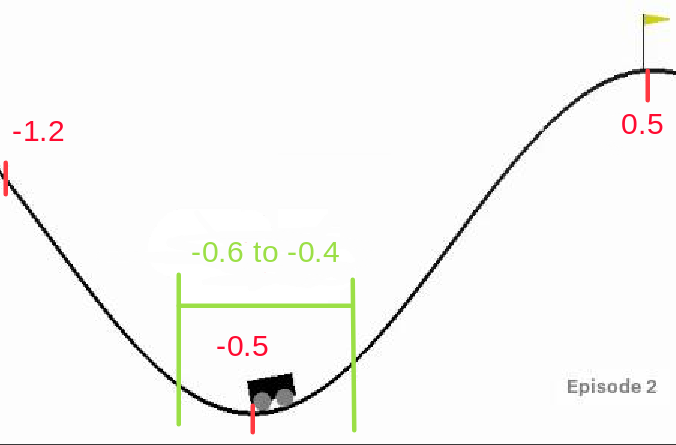
\includegraphics[width=0.8\textwidth]{env_data_visualization.png}
\caption{\label{fig:car_not_normalized} Mountain Car environment key positions}
\end{figure}

On the other hand, as shown in Table\ref{tab:1} velocity's range for the car is from -0.07 and 0.07 thus we can spot out an evident possible issue. Since both the velocity and position are the two variables fed to the deep neural network it is important that both are normalized as explained in this \href{https://www.coursera.org/lecture/deep-neural-network/normalizing-inputs-lXv6U}{video}. Normalizing the data input fed to the deep neural network will enhance optimality of the algorithm since fewer steps for the gradient descent in the loss function will be required as illustrated in Figure\ref{fig:NormVSnotNorm}. Where on the left we can note the function when a data input is not normalized and where is harder for the gradient descent to reach the global minimum, whereas at the right we could observe the function of the same data but this time normalized and in which clearly the gradient descent reaches the minimum smoothly.    

\begin{figure}[h]
\centering
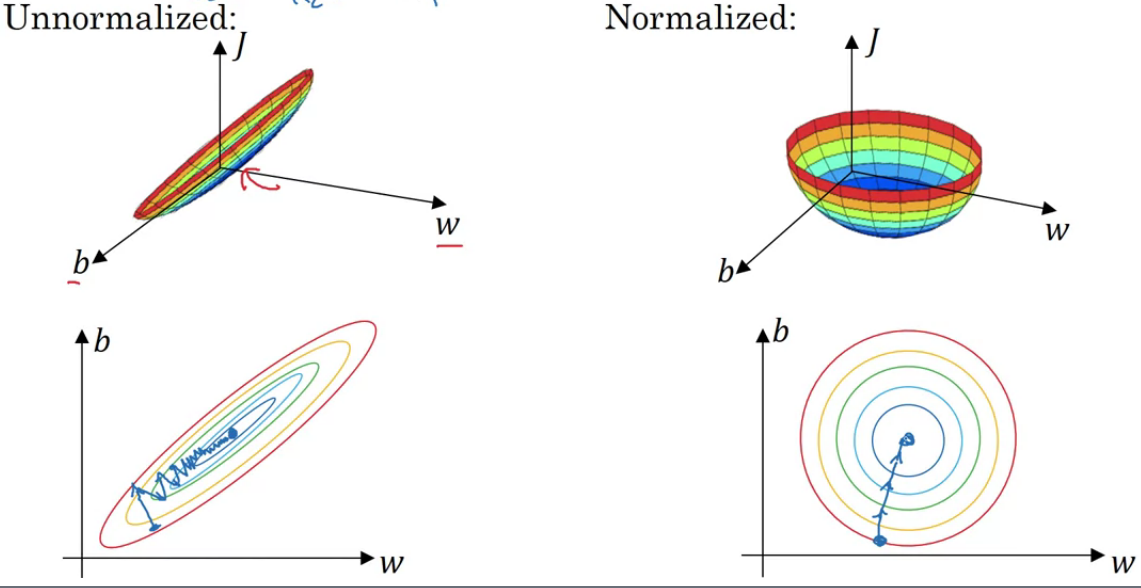
\includegraphics[width=0.8\textwidth]{normalizedVsUnnormalized.png}
\caption{\label{fig:NormVSnotNorm} Unnormalized vs Normalized data \cite{normalizing}}
\end{figure}

%%%%%%%%%%%%%%%%%%%%%%%%%%%%%%%%%%%%%%
\subsection{Deep Q Learning algorithm}
\label{sub:DQN}
%%%%%%%%%%%%%%%%%%%%%%%%%%%%%%%%%%%%%%
% Algorithms and techniques used in the project are thoroughly discussed and properly justified based on the characteristics of the problem. 
As stated in \href{https://storage.googleapis.com/deepmind-media/dqn/DQNNaturePaper.pdf}{DeepMind's paper} the Deep Q Network algorithm should be adequate for any problem where the state space is continuous and the action space discrete. The DQN should follow the following structure:
\begin{itemize}
\item Initialize replay Memory with capacity N
\item Initialize Main Q-network weights $W$ with random uniform distribution.
\item Initialize Target Q-network weights with the main Q-network weights. $W^-\leftarrow W$
\item \textbf{For} the episode in a maximum number of (Episodes):
\begin{itemize}
\item Reset environment
\item Prepare initial state: $S$
\item \textbf{For} time step t in a maximum number of (Steps):
\begin{itemize}
\item[] \underline{\textbf{Observation stage (sample to memory)}}
\item Act in the environment based on state $S$ and get action $A$ using an epsilon-greedy algorithm
\item Take action $A$ and make an environment action-step, get from the output of the environment the new state $S'$ and reward $R$
\item Store the tuple ($S,A,R,S'$) in memory
\item update state. $S \leftarrow S'$
\item[] \underline{\textbf{Learning stage }}\textbf{\dots} 
\item Obtain random mini-batch of tuples from memory. list of ($S,A,R,S'$).
\item Use Target Q-Network to predict the target $Q$ for Main Q-Network for each tuple of the mini-batch. 

$\hat{Q}$=predict($S$)

$\hat{Q}[A]=R+\gamma argMax_a(Q[S',W^-])$
\item Update weights in the Main Q-Network based on the target $\hat{Q}$ as follows: 

$\Delta W=\alpha (Q-\hat{Q}) \nabla_W(\hat{Q})$
\item Update Target Q-network weights with the Main Q-network weights every C steps. $W^-\leftarrow W$
\end{itemize}
\end{itemize}
\end{itemize}

%%%%%%%%%%%%%%%%%%%%%%
\subsection{Benchmark}
\label{sub:Benchmark}
%%%%%%%%%%%%%%%%%%%%%%
% Student clearly defines a benchmark result or threshold for comparing performances of solutions obtained. 

The project has been compared against three benchmarks:
\begin{itemize}
\item \textbf{Random approach}, to ensure the model is better than the most basic model.
\iffalse
\item \textbf{-110 average rewarding}, as stated in \href{https://github.com/openai/gym/wiki/Leaderboard#mountaincar-v0}{OpenAI's documentation} for the MountainCar-v0 the problem pass criteria is a reward of -110 in 100 consecutive episodes
\fi
\item \textbf{Leader board}, as explained in \href{https://github.com/openai/gym/wiki/Leaderboard#mountaincar-v0}{OpenAI's documentation} there are two algorithms that met the -110 average rewarding criteria as shown in Table\ref{tab:crit}. 

\begin{table}[h]
\centering
\begin{tabular}{|c|c|}
\hline
\textbf{User}      & \textbf{Episodes before solve} \\ \hline
jing582            & 1119                           \\ \hline
DaveLeongSingapore & 1967                           \\ \hline
\end{tabular}
\caption{Leader board for the MountainCar-V0 problem}
\label{tab:crit}
\end{table}

\end{itemize}